\documentclass[11pt]{book}
\usepackage[hidelinks]{hyperref}
\usepackage{float}
\usepackage{graphics}
\usepackage{pdfpages}
\usepackage{graphicx}
\setcounter{tocdepth}{3}
\setcounter{secnumdepth}{3}


\title{Social Theory Design Thinking}
\begin{document}
\maketitle
\tableofcontents


\part{Lecture Note.}
	\chapter{Week 1. Day 1.}
			\paragraph{05 August 2025.}
		\section{Syllabus.}
			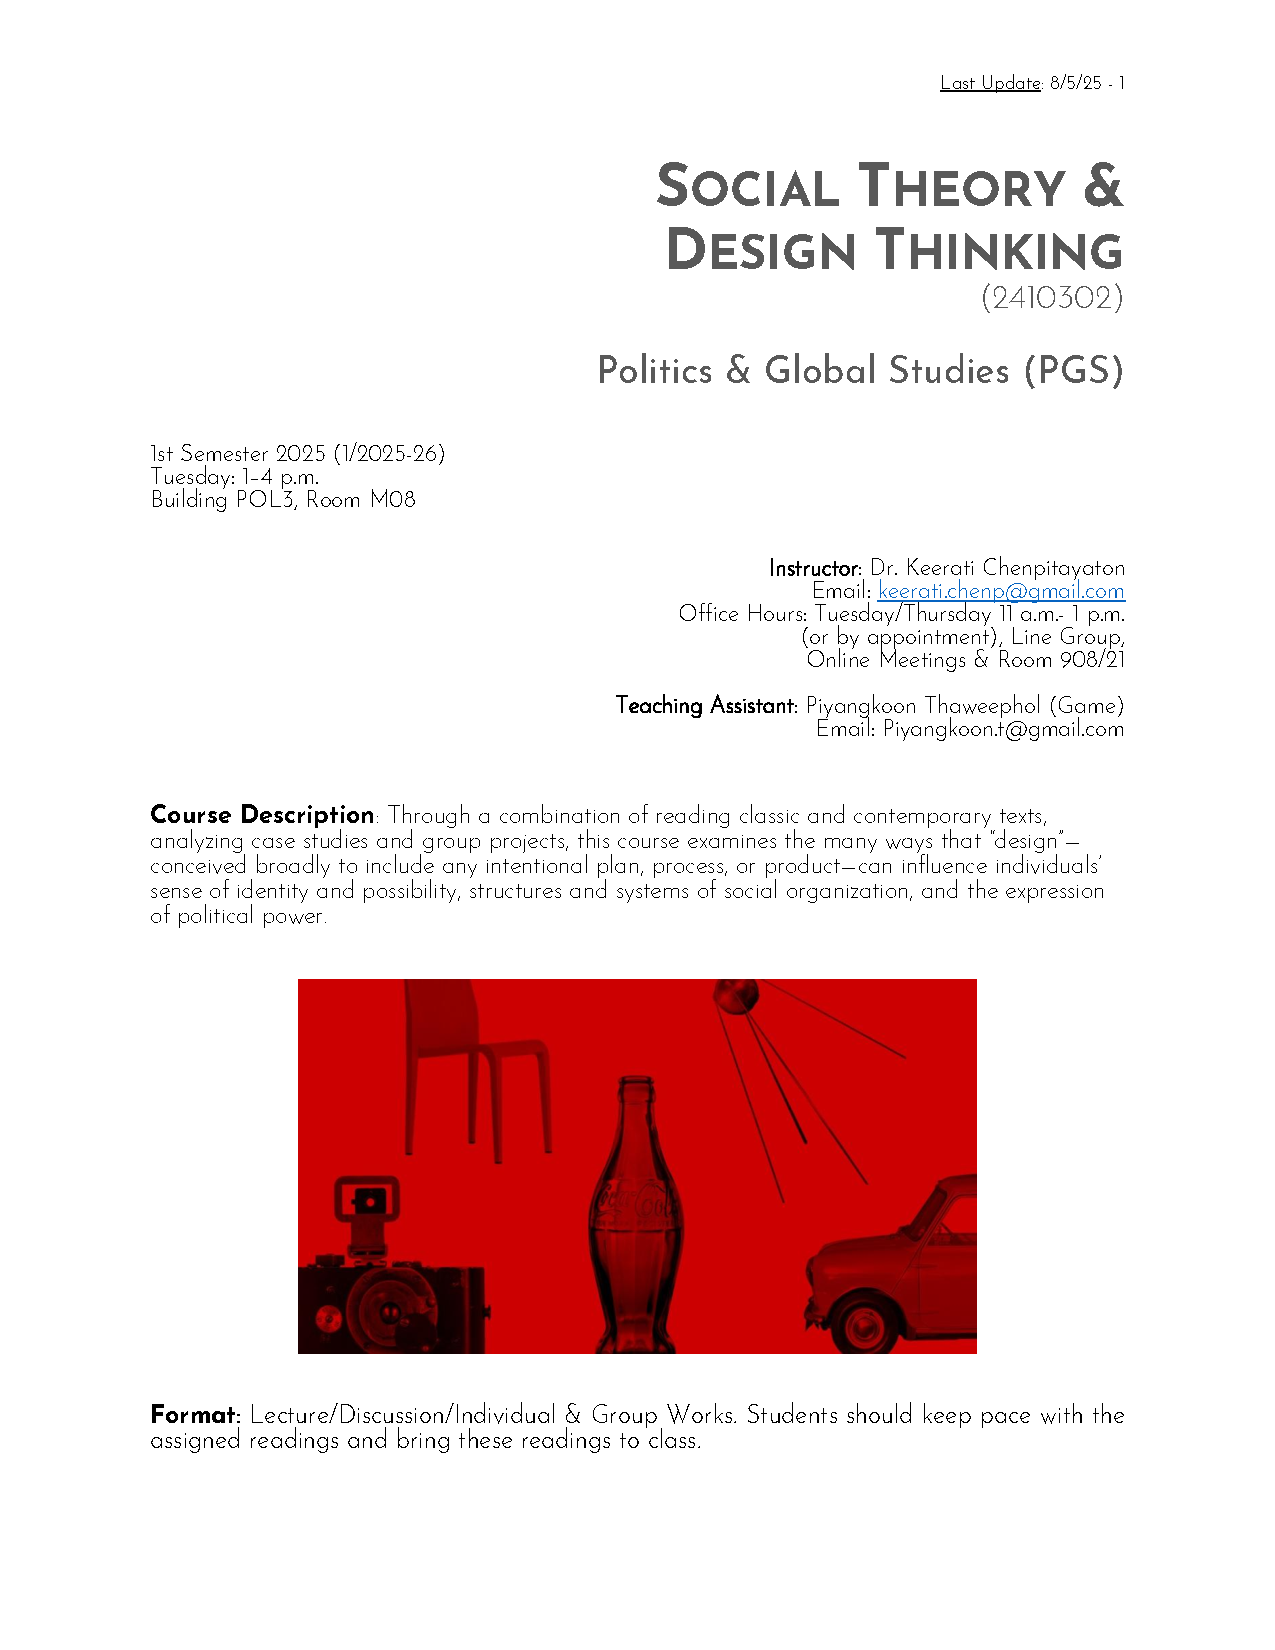
\includepdf[page=-]{Materials/ST&DTF25_PGSSyllabusTemporary.pdf}
			
			
\pagebreak
		
		
		\section{Group Exercise.}
				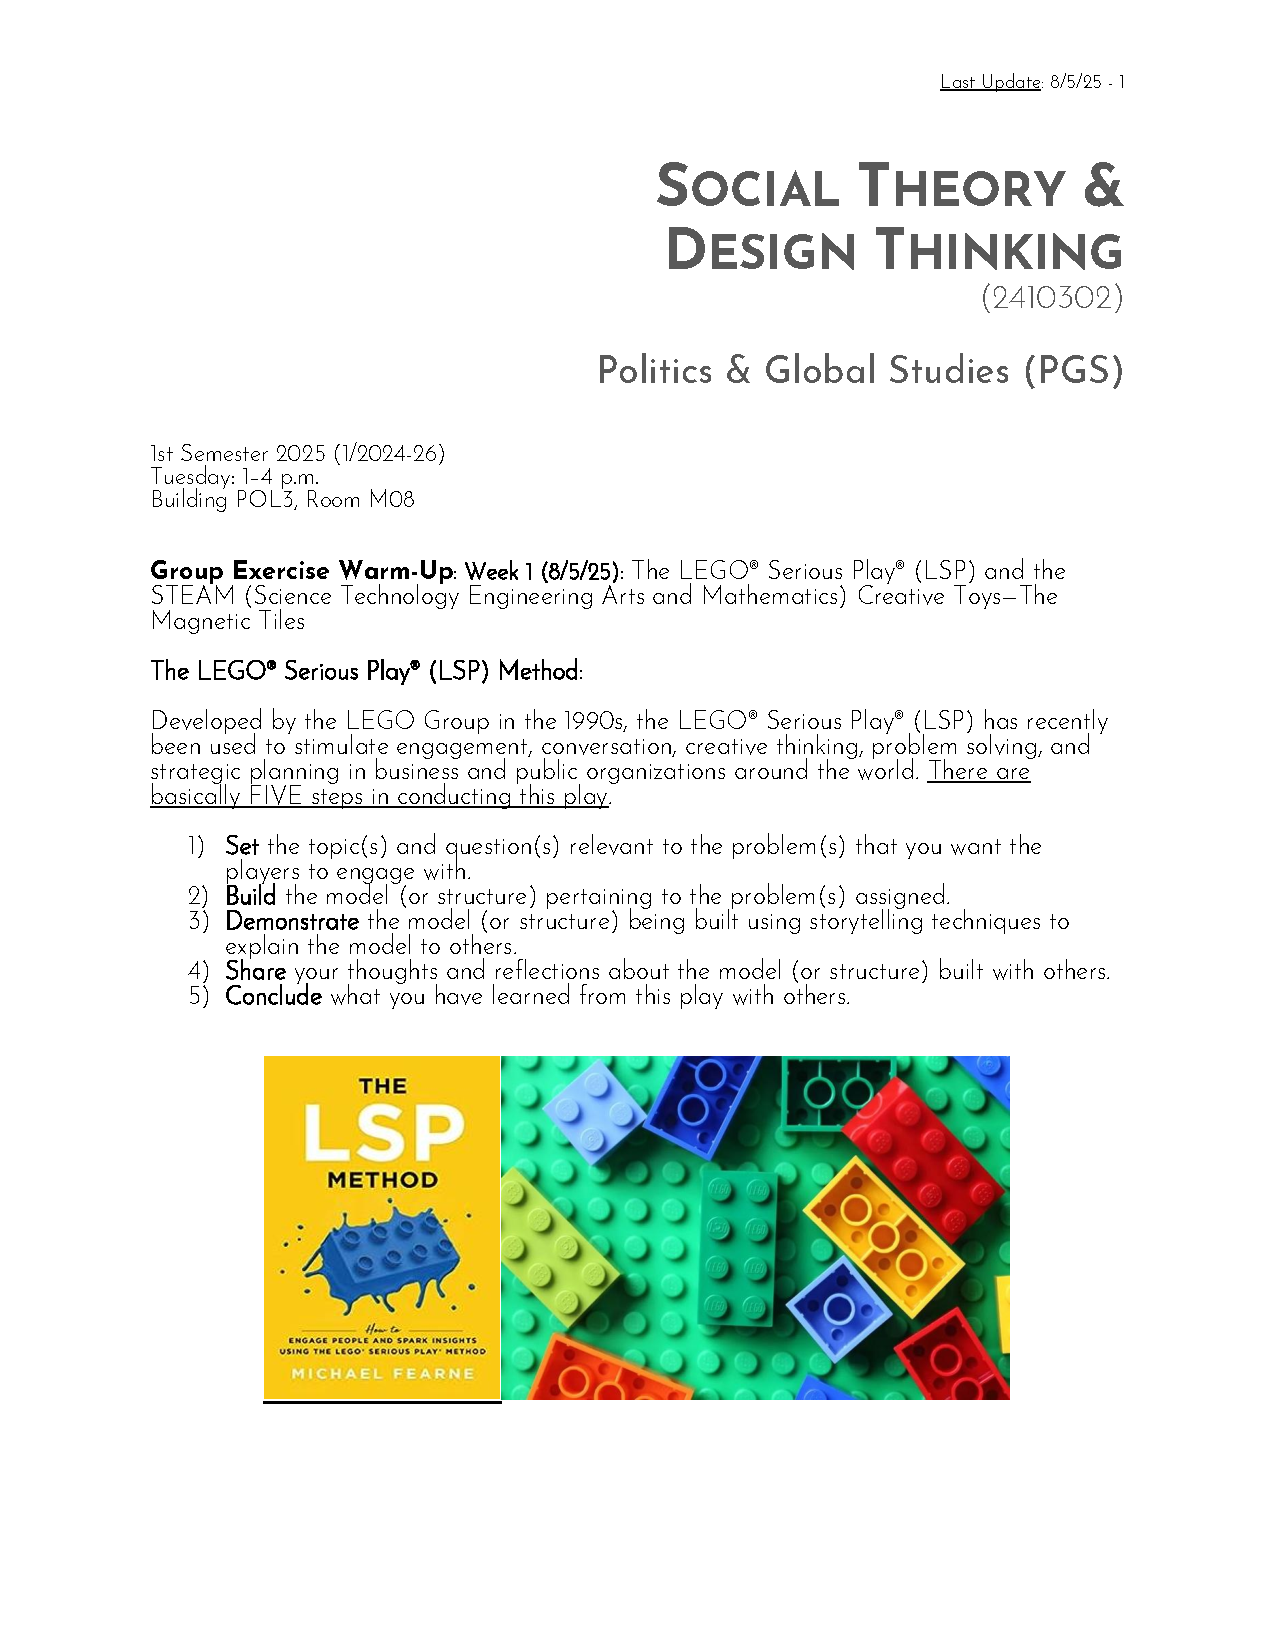
\includepdf[page=-]{Materials/STDTF25_W1&2GroupExercise.pdf}
		
			\subsection{Group Exercise Warm-Up.}
				\subsubsection{Task.}
				 Please get into the groups of 4-5 members for the total of 12 groups. Your group members will likely stay the same for the entire semester for the other group exercises throughout the course. Then, follow the instruction below. You have the total of 1.30 hrs. to finish the entire process through the five steps of the LSP method specified above. After that, we will go around the room and chit-chat with all groups. It’s an ice-breaking session for us to get to know each other and for you all to reflect on your teams’ experiences at the end of the course. Be relaxed and let your imagination run free!
				 
				\subsubsection{Procedure.}
					\begin{enumerate}
						\item Set the topic(s) and question(s) relevant to the problem(s) that you want the players to engage with.
						\item Build the model (or structure) pertaining to the problem(s) assigned.
						\item Demonstrate the model (or structure) being built using storytelling techniques to explain the model to others.
						\item Share your thoughts and reflections about the model (or structure) built with others.
						\item Conclude what you have learned from this play with others.
					\end{enumerate}
					
				\subsubsection{Work.}
						\textcolor{red}{NOTE: In Class Ice-Breaking.}
			\subsection{Assignment 1: Design for Mobility.}
				\subsubsection{Task.}
				In a world increasingly connected through daily crossings of borders, transportation of resources, and the spread of ideas and knowledge, mobility has become a pressing issue. Using the Mideer Distinctive Magnetic-Tiles: The 100 Pieces Set provided, design and construct a vehicle or transport-related object. Your design must address one of the following goals (please choosing only one):
					\begin{itemize}
						\item Increase accessibility for people with disabilities
						\item Reduce environmental impact
						\item Solve a specific mobility issue in your community (e.g., traffic, last-mile transport)
						\item Enable mobility in a difficult environment (e.g., desert, flood zones, war zones)
					\end{itemize}
				
				\subsubsection{Procedure.}
					\begin{enumerate}
						\item Collaborate to ideate, sketch, and build a prototype using the tiles.
						\item Name your design and describe its function, users, and impact in a short (2-minute) group presentation.
						\item Reflect briefly (in writing) on how your design reflects social needs and how design choices were made.
					\end{enumerate}
					
\newpage
					
				\subsubsection{Group 2: Work.}
					\paragraph{Topic:}
						Enable mobility in a difficult environment (e.g., \textcolor{red}{desert}, flood zones, war zones)
						\begin{figure}[H]
							\begin{center}
  							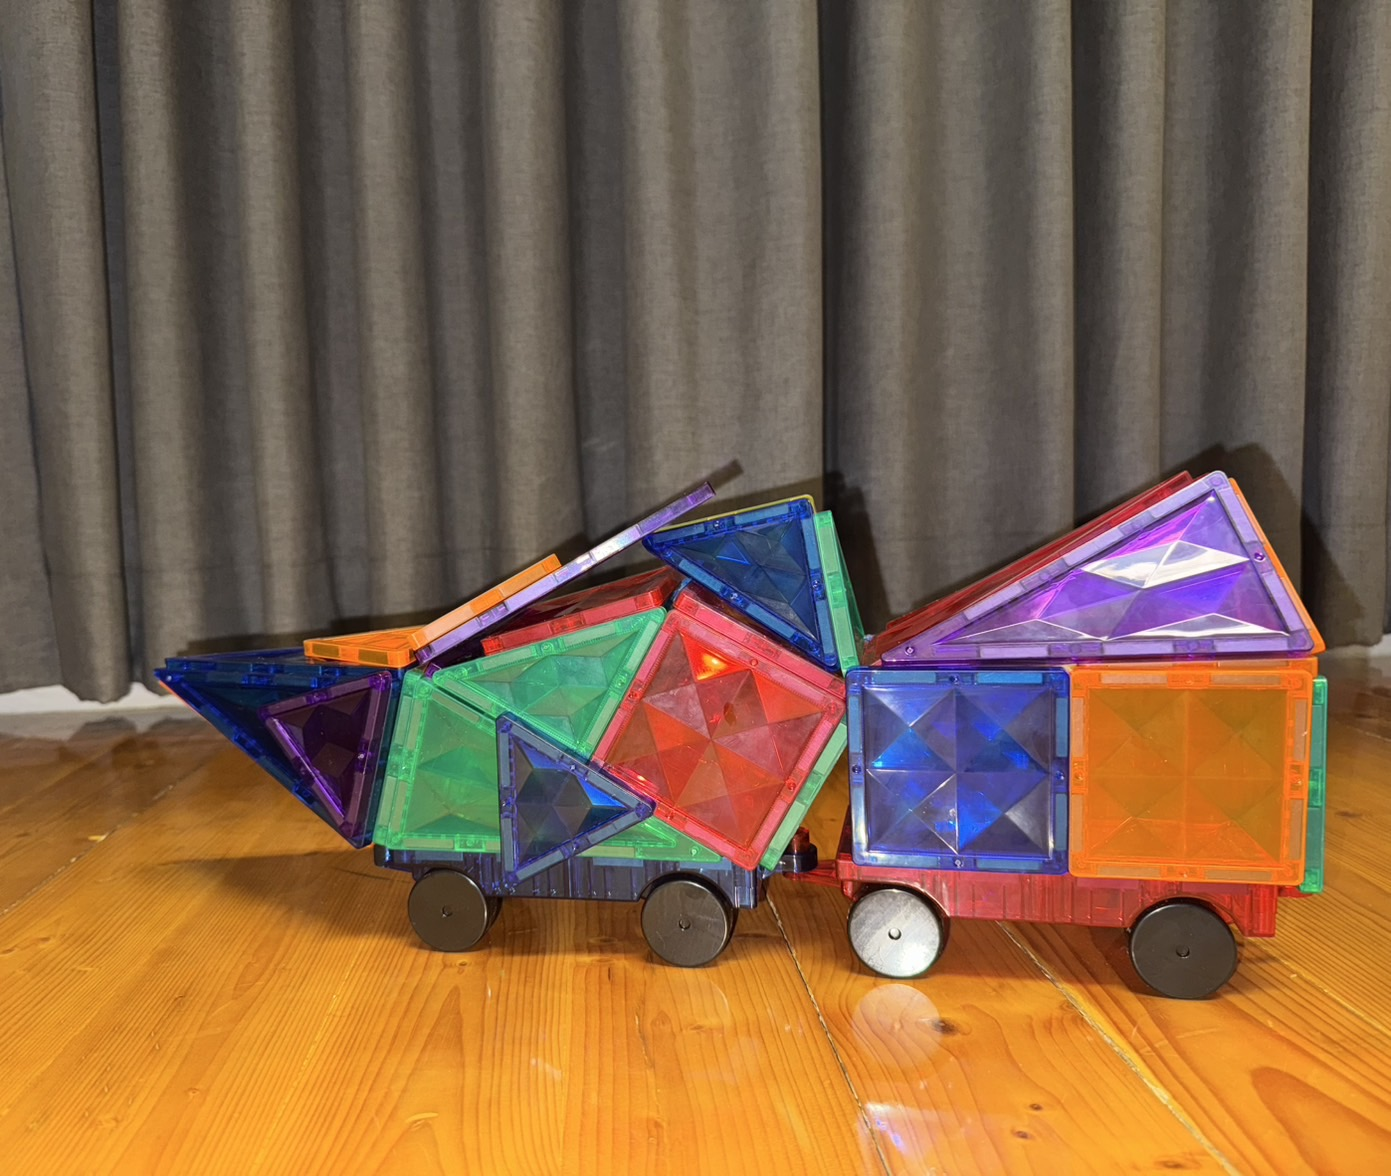
\includegraphics[scale=0.2]{Materials/S__41934851}
  							\end{center}
 							\caption{Sharky.}
						\end{figure}

					\paragraph{Name, Function, and Impacts.}
						\begin{itemize}
							\item Name:
								\subitem Sharky.
							\item Function:
								\subitem A special type of bus that specialised in transporting vast about of people in the desert environment.
								
								Sharky composed of:
									\begin{enumerate}
										\item Drill head.
											\subitem Use for drilling, and opening a path way, that may be difficult to normal mean of transportation.
										\item Coach.
											\subitem Sharky has an interlock system for it's coaches, allowing more capacity for a trip.
										\item Solarcell.
											\subitem Sharky is designed for  a long trip in the harsh environment such as desert; this solar cell act as an alternative fuel.
										\item Hydraulic Suspension System.
											\subitem  In the case that Sharky got stuck in a scenario that it cannot be move, Sharky can use it's Hydraulic Suspension System to sway, and jump out of the tight spot.
									\end{enumerate}
							\item Impacts:
								\subitem Sharky allows more mobility in the harsh environment--in this case, a desert--which can be further adapt into many mission. Whether it's to be means to transport citizens, helping or rescuing people in needs,  or transporting goods and materials.
						\end{itemize}
						
					\paragraph{Reflect:}
						
\newpage


		\section{Book: The LSP Method: How to Engage People and Spark Insights Using The LEGO Serious Play Method.}


	\chapter{Week 2. Day 1.}
			\paragraph{12 August 2025 \textcolor{red}{NOTE: NO CLASS}.}
	
			
	\chapter{Week 3. Day 1.}
	
\part{Homework.}


	\chapter{Week 1. Day 1.}
				\textcolor{red}{NOTE: NO HOMEWORK.}

	\chapter{Week 2. Day 1.}	
			\section{Assignment 2: Dystopia Design Challenge.}
				\textcolor{red}{To Be Completed as Your Homework before Week 3: 19/08/2025.}
			\subsection{Task.}
				Imagine your group is living in a dystopian future where society has drastically changed (due to climate collapse, authoritarian rule, extreme inequality, AI takeover, etc.). Design a socio–technical structure or system using the Mideer Magnetic-Tiles: The Marble Run Set that helps people survive or resist within this dystopia.
				
			\subsection{Procedure.}
				\begin{enumerate}
					\item Define your dystopian world: What happened? Who has power? What are the living conditions? (Write a short paragraph and put it in your group portfolio; see below.)
					\item Build a prototype of socio–technical structure or system that helps with survival, rebellion, communication, or adaptation.
					\item Take some digital photos of your design. Present your design by writing short paragraphs and put them in your group portfolio (see below), explaining:
						\subitem The context of the dystopia
						\subitem The purpose and function of the design
						\subitem Ethical questions or trade-offs the design raises
					\item Reflect briefly (in writing) on how design can both oppress or empower in times of crisis.
				\end{enumerate}
				
				
		\section{Week 2 (12/08/2025): Individual, and Group's Free Writing Exercise.}
			\textcolor{red}{To Be Completed as Your Homework before Week 3: 19/08/2025.}
			\subsection{Task.}
			For each group’s member, please write (either handwriting or typewriting) only 1-2 pages introducing yourself to us. This introduction should at least include your biographical history such as what school you went to, what would be your future career, and why you want to come to pursue a degree with PGS, etc. An illustration in terms of your photo will be highly appreciated in order for us to remember you throughout the course.
			
			Then, please assemble all of your group members’ self-introduction into one group portfolio. The portfolio should include your team’s reflection of the dystopia design challenge.
			\linebreak
			
			\textbf{Last Update: 8/5/25 - 5}
			
			Even though you will have one week off because Week 2’s meeting is a national holiday (Mother’s Day; Tuesday, 8/12/25), we suggest that you spend only an hour or two on this exercise, as your group members get together to assemble everything into a group portfolio. Submit a PDF digital copy by uploading it into Week 1’s folder in this year’s course Google Drive before the next two weeks’ meeting: Week 3: 8/19/25
\part{Course Summary.}
	\chapter{Topic}

\end{document}
